%\documentclass[referee]{aa} % for a referee version
%\documentclass[onecolumn]{aa} % for a paper on 1 column  
%\documentclass[longauth]{aa} % for the long lists of affiliations 
%\documentclass[letter]{aa} % for the letters 
%\documentclass[bibyear]{aa} % if the references are not structured according to the author-year natbib style

\documentclass{aa}  
\usepackage[polish]{babel}
\usepackage[T1]{fontenc} 
\usepackage[utf8]{inputenc}
\usepackage{graphicx}
\usepackage{txfonts}
\usepackage{amsmath}
\usepackage{graphicx}
\usepackage{gensymb}
\usepackage{subcaption}
\usepackage{amsmath}
\usepackage{url}
\usepackage{hyperref}

\begin{document}

   \title{Identification of sdBV star pulsed modes}
   \subtitle{}
   \author{Radosław Kluczewski \inst{1}}
    \institute{Faculty of Physics, Astronomy and Applied Computer Science of the Jagiellonian University \\
        \email{radek.info.klucz@gmail.com}
             }
\abstract
  % context heading (optional)
  % {} leave it empty if necessary  
   {} 
  % aims heading (mandatory)
 {Obtaining a list of pulsed frequencies of an sdBV star with quantum numbers l, n, m.}
  % methods heading (mandatory)
   {The use of shared programs for calculating the Fourier transform and the python language for data processing.}
  % results heading (mandatory)
   {List of pulsed frequencies with period, amplitude and quantum numbers.}
  % conclusions heading (optional), leave it empty if necessary 
   {}
   \keywords{}
\maketitle
%--------------------------------------------------------------------
\section{Theoretical basics}

Pulsating stars are variable stars that change their brightness, size and shape periodically. Periodicity is related to the occurrence of a partial ionization layer in the outer regions of the star, which under certain conditions destabilizes the star by first contracting it and then expanding around the equilibrium position. Based on the observation of the frequency spectrum of the pulsations, astroseismology, i.e. the field of astrophysics that studies these pulsations and vibrations, is able to obtain information about the interior of the studied star.

Vibrations of the star gas occur in three dimensions, so theoretical description uses quantum integers \textbf{n}, \textbf{l}, \textbf{m}. The number \textbf{n} describes the radial order of magnitude of the mode, that is, it contains the number of nodal surfaces inside the star. These surfaces do not take part in the movement, only separating the layers in which the gas moves in different directions. The angular degree of the \textbf{l} mode gives information about the number of nodal planes on the star's surface, while the azimuth \textbf{m} degree gives information about the lines passing through the poles of the pulsating star. Node lines divide the star into regions where the physical conditions change as a result of pulsations in opposite phases (for example, changes in brightness).

When $ |m| \leq l $ then for a given module m describes the side lobe of the module located on the left and right sides (symmetrically) of the Fourier transform with respect to the central lobe. When a pulsating star is spherical and the slow rotation approximation is used, the multiplet mode frequencies are proportional to the star's rotation frequency. Thus, on the basis of the intervals between successive frequencies of the multiplet, the rotation of the star can be determined.
%--------------------------------------------------------------------
\section{Performing the exercise}

The sdB93.data file was used to perform the exercise, which contains data about the brightness curve of a pulsed star. Additionally, sources [1] and [2] were used during data compilation.

\subsection{Calculation of the Fourier transform from the selected brightness curve}

In order to perform the calculations, the \textit{jkft50} program, which calculates the Fourier transform, was used. The resulting file, after running the program, is the Fourierive amplitude spectrum, which includes frequency columns in [c/d] and frequency amplitudes in [ppt] units.

\subsection{Calculation of the noise level of the amplitude spectrum}

Using the \textit{ftnoise} program, the detection level ranging from 0 to 50 cycles per day was calculated, the value of which was: $ 0.037. $ The above result corresponds to a noise detection level of $ 4 \cdot \sigma $, where $ \sigma $ is the average noise floor of the Fourier transform. This result is marked in the picture \ref{fig:my_label_1}.  

\subsection{Spectrum signals identification}

The $ \textit{scipy} $ module and the $ \textit{find peaks} $ function were used to identify spectrum signals that exceed the noise level set. Additionally, a spectral window was generated by means of which the signals constituting artifacts of the Fourier transform were eliminated. The identified signals without artifacts are summarized in Table 1, with frequency and period recorded for each identified "peak".

The spectral windows are presented in the picture \ref{fig:my_label_2} and the picture \ref{fig:my_label_2_o}. To draw the spectral window, it was necessary to prepare a sinusoid for points with the same time distribution as for the sdB93 data, which will be used to identify multiplets and triplets (m numbers for a given l).Next, the Fourier transform was calculated for the generated sine wave, which was compared with the signals with the highest amplitudes, close to which the possible components of the multiplets also have high amplitudes. From the spectral window, it is possible to determine which signals are artifacts. After eliminating the mentioned artifacts, we are able to correctly identify the true components of multilipets (if they exist).

\subsection{Converting the $ f_i [c / d] $ frequency list to $ P_i [s] $ periods}

The signals found along with the entire sdB93 data range were converted from frequency in units of cycles per day to periods in seconds. The conversion formula is presented below: $$ \frac{86400}{i}, $$ where the number 86400 is a day expressed in seconds, and i is the frequency from the data transform. The signals in the periods are listed in Table 1 and in fig.\ref{fig:my_label_3}, which shows the amplitude spectrum of the Fourier transform as a function of the period in seconds. Additionally, in the picture \ref{fig: my_label_30} the so-called mod ladder is presented, i.e. the fourier transform amplitude spectrum plotted with the equidistant dots of the mods $ l_1 $ (272.62 seconds, green color), $ l_2 $ (151.92 seconds, blue color) ) and $ l_3 $ (78.23 seconds, black). The ladder was developed with the help of the identified modes shown in fig.\ref{fig:my_label_2} and fig.\ref{fig:my_label_2_o}. From the figures cited, the central frequencies of the peaks were read, which were the starting points for the equidistant dots. Then, successive dots were plotted for a given number l = 1 and l = 2 with distances equal to 272.62 seconds and 151.92 seconds, respectively, on both sides of the center mode frequency, until the entire range of the Fourier transform is filled.

\subsection{Finding the distance $ \ Pi_ {l_1} $, $ \ Pi_ {l_2} $ for the $ l_1 $ and $ l_2 $ series}

For pulsating stars, the sdBV in the space of the pulsation mode periods for a given l are approximately equal spacing. The distance between the \textit{n} and \textit{$ n + 1 $} modes is approximately 245 seconds for $ l = 1 $ and 140 seconds for $ l = 2 $. For the modes defined in this way, the data was divided by assigning them the values of $ l_1 $ and $ l_2 $ in advance in order to obtain transparent histograms. Initially, the data was divided into parts with periods $ T <$ 4500 and $ T> $ 4500, where a distance of 245 seconds was expected for the first range, and 140 seconds for the second. This solution did not bring the expected results because it eliminated a significant part of the distance between the signals. Ultimately, it was decided not to divide the data into two parts, but to calculate the distance for the entire data range without pre-assignment. Then, using the python language, the $ \textit{math} $ module and the $ \textit{dist} $ function, the distances to be searched were calculated. The formula for calculating the distances is presented below:

\begin{equation}
    d(x_i, x_j) = |(x_i - x_j)|,
\end{equation}

where $ x_i $ and $ x_j $ are respectively x coordinates of the identified signals expressed in periods. fig.\ref{fig:my_label_4} presents a histogram of the distribution of the occurrence of a given distance from the distance between the signals. As you can see, the plotted distance histogram for the data has successive mods in the distance $ n \cdot \Pi $, where $ \Pi $ is the distance for a given l. 


\subsection{Identification of mods}

To identify the modes, a histogram was used for the entire data with a bar width of 12 seconds, fig.\ref{fig:my_label_4}, to which Gaussian functions were fitted, where the fields under the graph were normalized to one. The intervals for fitting Gaussian functions are respectively for Fig.\ref{fig: my_label_6} with a bar width of 3 seconds and for fig.\ref{fig:my_label_7} with a bar width of 4 seconds, intervals of 120 - 190 seconds and 240 - 300 seconds. The fit parameters are:

\begin{itemize}
    \item $\mu_{l_1} = 272.62,$
    \item $\sigma_{l_1} = 5.82,$
    \item $\mu_{l_2} = 151.92,$
    \item $\sigma_{l_2} = 8.01.$
\end{itemize}

For the matching parameters thus obtained, the modes of individual signals were then identified, where the identification of a given mode was based on the following histogram width ranges:
   $$ ( \mu_2 - \sigma_2, \mu_2 + \sigma_2 ). $$ 
If modes giving such a space were found in a given interval of intervals, then the mod was identified as $ l_1 $ (the first range) or $ l_2 $ (for the second range).

Additionally, in the histogram for the totality of the data in fig.\ref{fig:my_label_4} one can see a small maximum corresponding to the distance between the periods of approximately 80 seconds, which may correspond to the intervals between the periods for $ 1 = $ 3. For these distances, the Gaussian function was also fitted fig.\ref{fig:my_label_11}, where the width of the histogram bars is 3 seconds with the following interval 70 - 90 seconds and parameters: 

\begin{itemize}
    \item $\mu_{l_3} = 78.23,$
    \item $\sigma_{l_3} = 1.51,$
\end{itemize}

Then the modes were identified in the same way as above. The results of all identified modes are presented in Table 1.

The justification for the distance of approximately 80 seconds results from the following formula taken from publication [3], where the distance between the modes with l = 3 is described as follows:

\begin{equation}
    DP(l=3) = \frac{1}{2} \cdot DP(l=1).
\end{equation}

In the above formula, DP (l = 1) is the distance between modes for l = 1. So for l = 1 of approximately 150 seconds we are able to assign a peak l = 3 of approximately 80 seconds.

The number n describing the radial row has also been identified. This number was assigned to $ l = 1$  and $ l = 2$  starting at $ n = 1$. When the identified signals expressed in periods are 272.62 seconds and 151.92 seconds apart, they are assigned relative values of n, respectively, where for the next equidistant signal the number of the radial order will be $ n = n_{current} + 1$. The missing equidistant mod in the sequence increases n by 1, so there are also gaps not assigned a number of n between the periods. Table 1 shows the identified radial order number n with the expected gaps.

\subsection{Visual identification of multiplets}

In order to confirm the identification from the so-called mode ladder fig.\ref{fig:my_label_30} visual identification of the multiplets was made. Thus, for the modes with the highest amplitudes, multiplet components were found, where $ | m | \ leq l. $ Examples of identifications are presented in the picture \ref{fig:my_label_2} and in the picture \ref{fig:my_label_2_o}. As can be seen in the first figure, we can see symmetrical signals with respect to the centered peak for $ 1 = 2$, which protrude above the detection level, and the drawn sine wave. These signals were respectively identified as $ m = -2, -1, +1, + 2$ . Similarly, visual identification was carried out in the second figure, which shows the central signal for l = 1 with the detection level plotted and the fitted sinusoid. Identified symmetrical signals projecting above the detection level and sine waves are described by the following numbers $ m = -1, + 1 $. All identified m numbers are presented in Table 1.

\subsection{Designation Confirmation $\Pi$}

In order to confirm the determination of $ \Pi $, the Fourier transform was calculated from the amplitude spectrum but converted to period. Before performing the calculations, using the \textit{jkft50} program, the range of the Fourier transform was limited to 20,000 seconds and sorted in ascending order with respect to the period column. For the data prepared in this way, the transform was calculated, the results of which are presented in fig.\ref{fig:my_label_8}. By comparing the graph with the obtained maxima of the histograms in frequencies, which were marked in the above-mentioned figure, respectively $ \sigma_1 = 1 / 151.92 $ and $ \sigma_2 = 1 / 272.62 $, you can try to confirm the correctness of determining the distance between the mode series periods for a given l, which should be seen in the Fourier transform from the period-converted amplitude spectrum.

%--------------------------------------------------------------------
\section{Discussion of the results}

By using the python programming language, it was possible to identify the $ l_1 $, $ l_2 $ and $ l_3 $ modes. It is also worth noting the number of peaks identified, the number being 130. This is the expected number of peaks for sdBV stars. The larger number was due to the use of a programming language function that counts all signals and artifacts above a predetermined detection level. Most of the artifacts were visually eliminated through the use of a spectral window. Attempts were also made to eliminate artifacts by including the $ \textit{prominence} $ filter in the $ \textit{find peaks} $ function, but no significant improvement was noticed for the histogram. The use of the filter cut the distance which resulted in fitting the Gaussian function for a small number of counts. As a consequence, it also influenced the correct identification of modes, where for the mentioned distance there were practically no identifiable numbers $ l = $ 1. Finally, it was decided to fit the Gaussian function for signals $ _{\textasciitilde} 80 $, $ _{\textasciitilde} $ 155, $ _{\textasciitilde} $ 270 for all data without applying a filter. The identification of the number of the radial order n confirms the assumption that there is a gap that does not have the assigned value of the number n. The visual identification of the number m confirmed the existence of multiplets. On the other hand, the maxima of the histograms for individual signals equal respectively: $ \sigma_1 = 1 / 151.92 $ and $ \sigma_2 = 1 / 272.62 $ coincide with the graph confirming the designation of $ \Pi $, so the identification of the mods was correctly made. By using the python programming language the $ l_1 $, $ l_2 $ and $ l_3 $ mods were identified. It is also worth noting the number of peaks identified, the number being 130. This is the expected number of peaks for sdBV stars. The larger number was due to the use of a programming language function that counts all signals and artifacts above a predetermined detection level. Most of the artifacts were visually eliminated through the use of a spectral window. Attempts were also made to eliminate artifacts by including the $ \textit{prominence} $ filter in the $ \textit{find peaks} $ function, but no significant improvement was noticed for the histogram. The use of the filter cut the distance which resulted in fitting the Gaussian function for a small number of counts. As a consequence, it also influenced the correct identification of modes, where for the mentioned distance there were practically no identifiable numbers $ l = 1$. Finally, it was decided to fit the Gaussian function for signals $ _{\textasciitilde} 80 $, $ _{\textasciitilde} $ 155, $ _{\textasciitilde} $ 270 for all data without applying a filter. The identification of the number of the radial order n confirms the assumption that there is a gap that does not have the assigned value of the number n. The visual identification of the number m confirmed the existence of multiplets. On the other hand, the maxima of the histograms for individual signals equal to $ \sigma_1 = 1 / 151.92 $ and $ \sigma_2 = 1 / 272.62 $, respectively, coincide with the graph confirming the designation of $ \Pi $, so the identification of the mods was correctly made.

\section{Reference}
\begin{enumerate}
\item Jerzy Krzesinski, 2015, A\&A 581, A7, 7
\item Radosław Smolec, Asterosejsmologia – probing the interior of stars, Astronomical Center for them. Nicholas Copernicus, Warsaw
\item J. Krzesiński, A. Blokesz, A.S. Baran, S. Bachulski, 2014, AA, 64, 151–165
\end{enumerate}

\begin{figure*}[h]
    \centering
    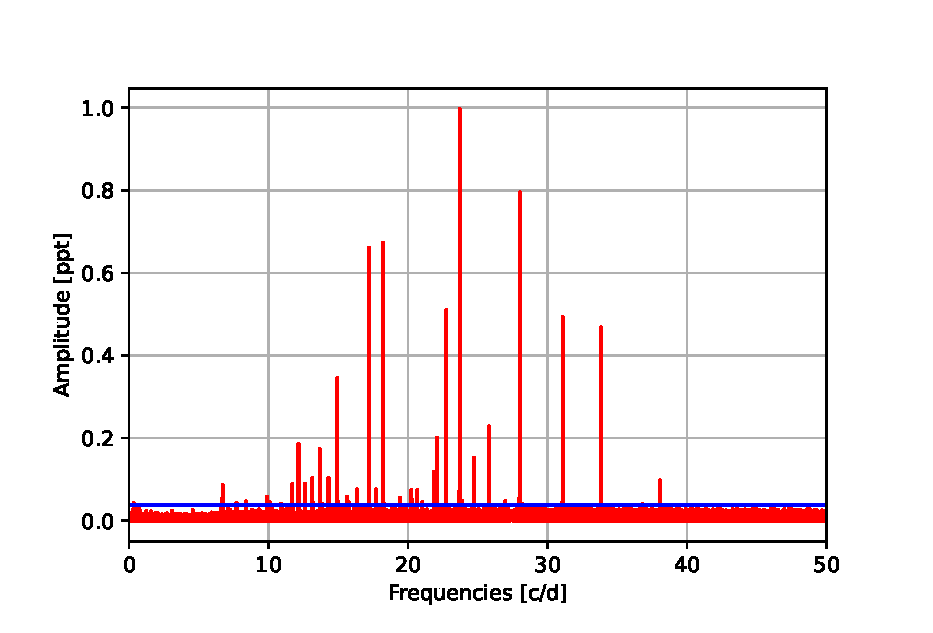
\includegraphics[scale=1]{images/transformat_fourier_frequencies_with_noise.eps}
    \caption{The amplitude spectrum of a pulsating star in red with the detection level in blue.}
    \label{fig:my_label_1}
\end{figure*}

\begin{figure*}[h]
    \centering
    \includegraphics[scale=0.6]{images/okno_spektralne.pdf}
    \caption{Spectral window superimposed on the pulsed mode with the frequency 18.203054 [c/d]. Apart from the main frequency, there are also visible weak multiplet signals, two on each side of the frequency 18.203054 [c / d] (ie 18.187281, 18.195129 and on the other side of the central peak 18.210979, 18.217905). Thus, the mod can be identified as $ l = 2 $, where red is the amplitude spectrum of the data, black is the generated sinusoidal amplitude spectrum, and blue is the detection level of the amplitude spectrum.}
    \label{fig:my_label_2}
\end{figure*}

\begin{figure*}[h]
    \centering
    \includegraphics[scale=0.58]{images/okno_poprawione_l1_to_l2.pdf}
    \caption{Spectral window superimposed on the pulse mode with the frequency 23.69969 [c / d]. Apart from the main frequency, there are also visible weak multlet signals, two on each side of the 23.69969 [c / d] frequency (ie 23.691763 and on the other side of the central peak 23.707615). Thus, the mod can be identified as $ l = 1 $, where red is the amplitude spectrum of the data, black is the generated sinusoidal amplitude spectrum, and blue is the detection level of the amplitude spectrum.}
    \label{fig:my_label_2_o}
\end{figure*}

\begin{figure*}[h]
    \centering
    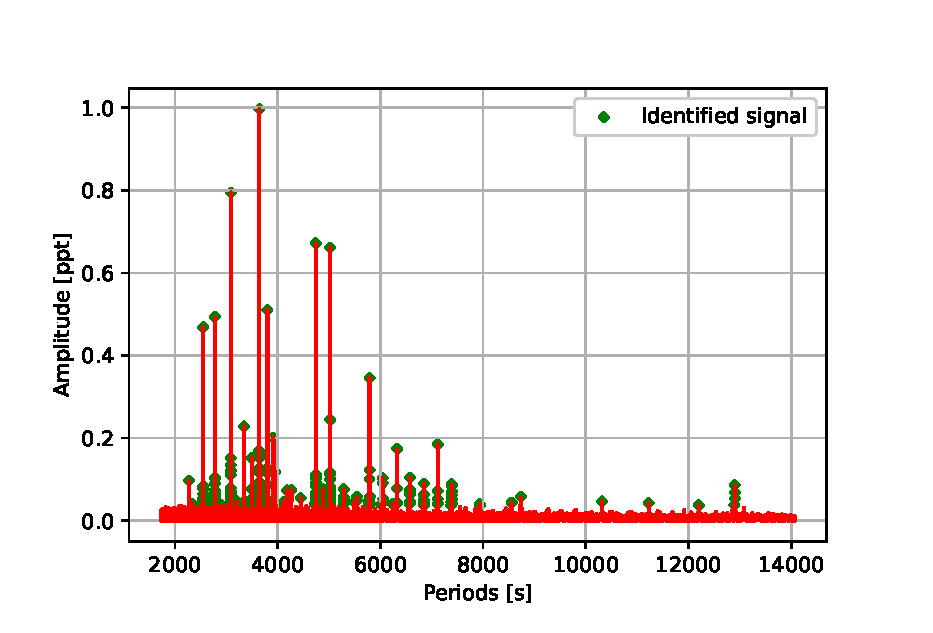
\includegraphics[scale=1]{images/identified_signal_in_period.eps}
    \caption{Converted (see 2.4) spectrum of the Fourier transform with plotted signals.}
    \label{fig:my_label_3}
\end{figure*}

\begin{figure*}[h]
    \centering
    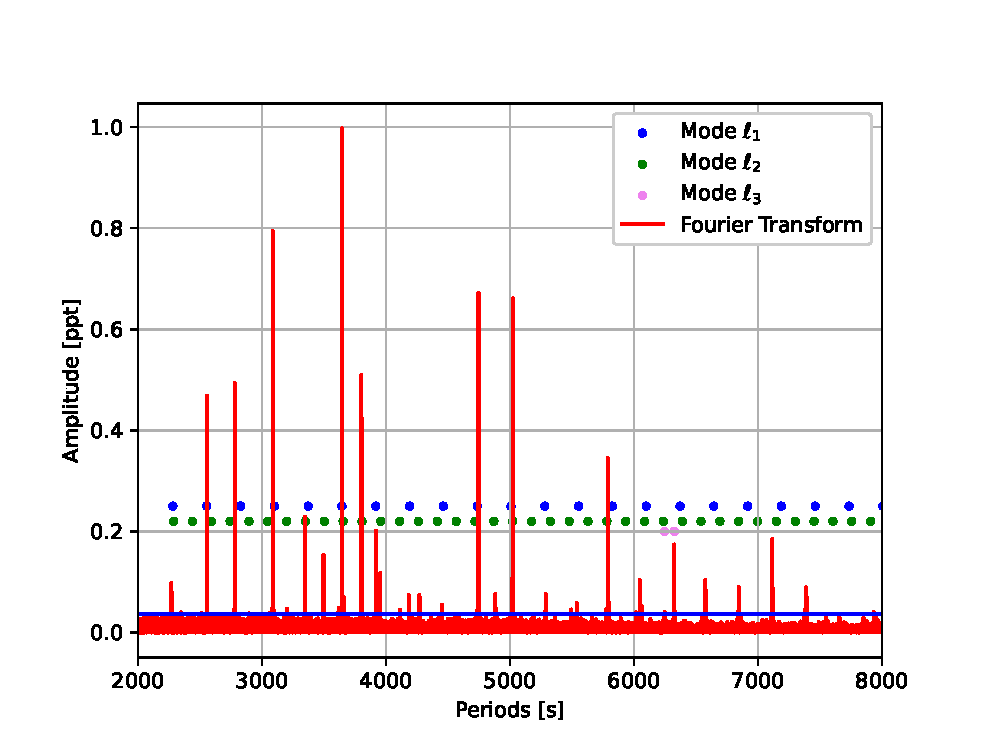
\includegraphics[scale=1]{images/ehhhhh.eps}
    \caption{Converted amplitude spectrum with plotted signal modes.}
    \label{fig:my_label_30}
\end{figure*}

\begin{figure*}[h]
    \centering
    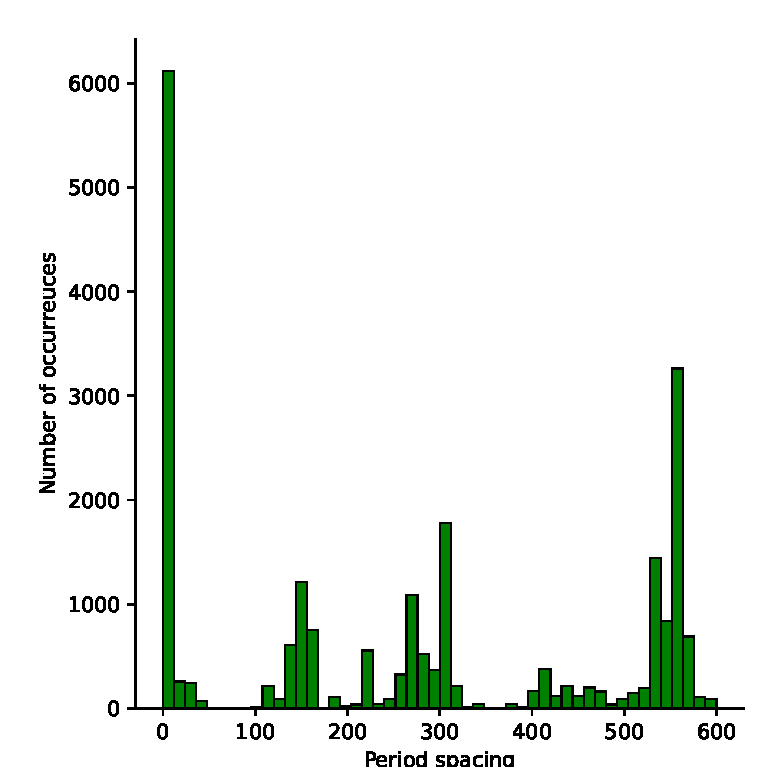
\includegraphics[scale=1]{images/his_all_data.eps}
    \caption{A histogram that shows the distance distribution for the data, where the bars are 12 seconds wide.}
    \label{fig:my_label_4}
\end{figure*}

\begin{figure*}[h]
    \centering
    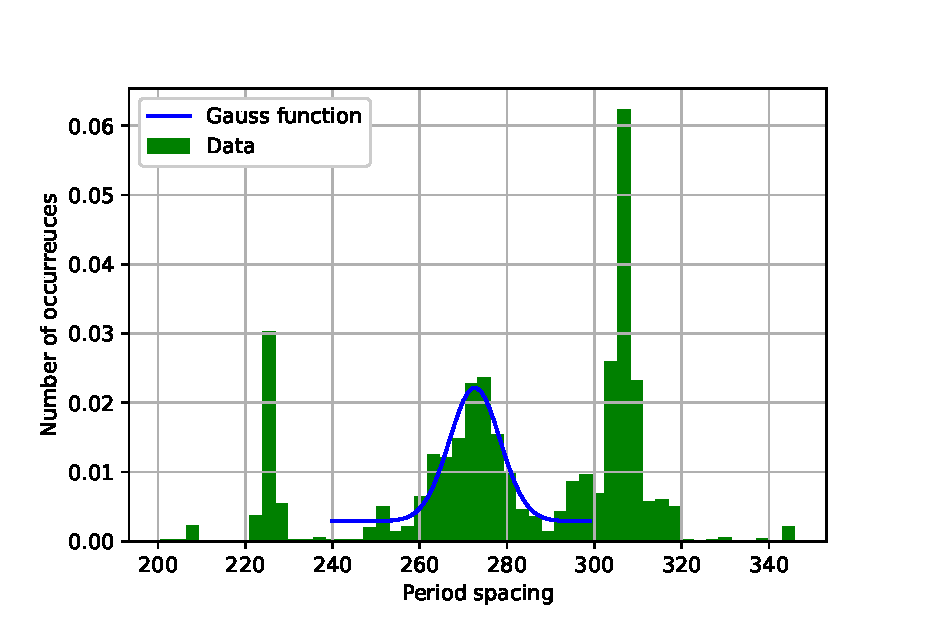
\includegraphics[scale=1]{images/histogram_l1_gauss.eps}
    \caption{Histogram showing the distance distribution for $ l = $ 1 with fitted Gaussian function in the range 240 to 300 seconds, where the bars are 3 seconds wide.}
    \label{fig:my_label_6}
\end{figure*}

\begin{figure*}[h]
    \centering
    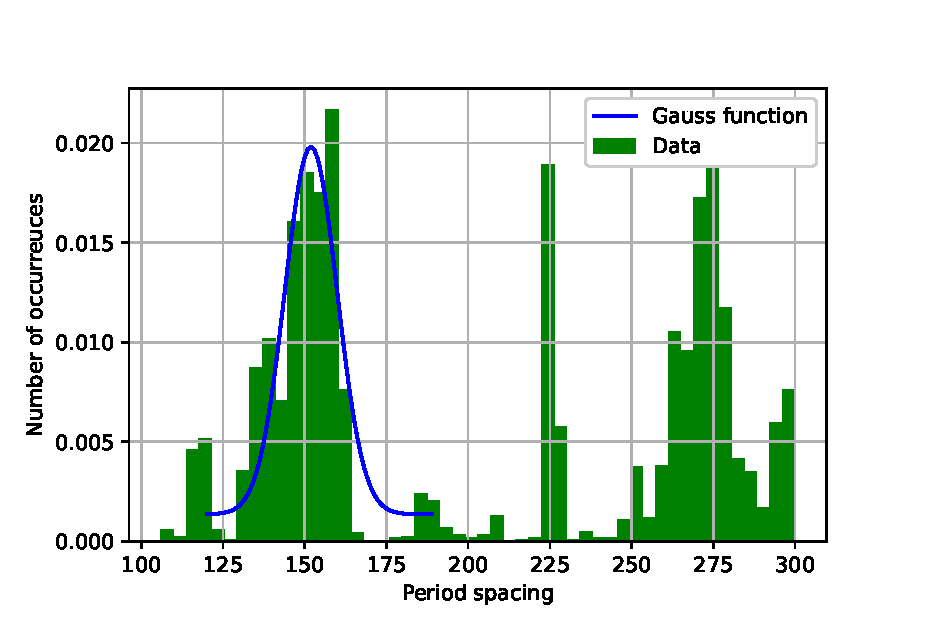
\includegraphics[scale=1]{images/histogram_l2_gauss.eps}
    \caption{Histogram showing the distance distribution for $ l = 2$  with fitted Gaussian function in the range from 120 to 190 seconds, where the width of the bars is 4 seconds.}
    \label{fig:my_label_7}
\end{figure*}

\begin{figure*}
    \centering
    \includegraphics[scale=1]{images/histogram_l3_gauss.eps}
    \caption{Histogram showing the distance distribution number for $ l = 3$  with fitted Gaussian function in the range from 70 to 85 seconds, where the width of the bars is 3 seconds.}
    \label{fig:my_label_11}
\end{figure*}

\begin{figure*}[h]
    \centering
    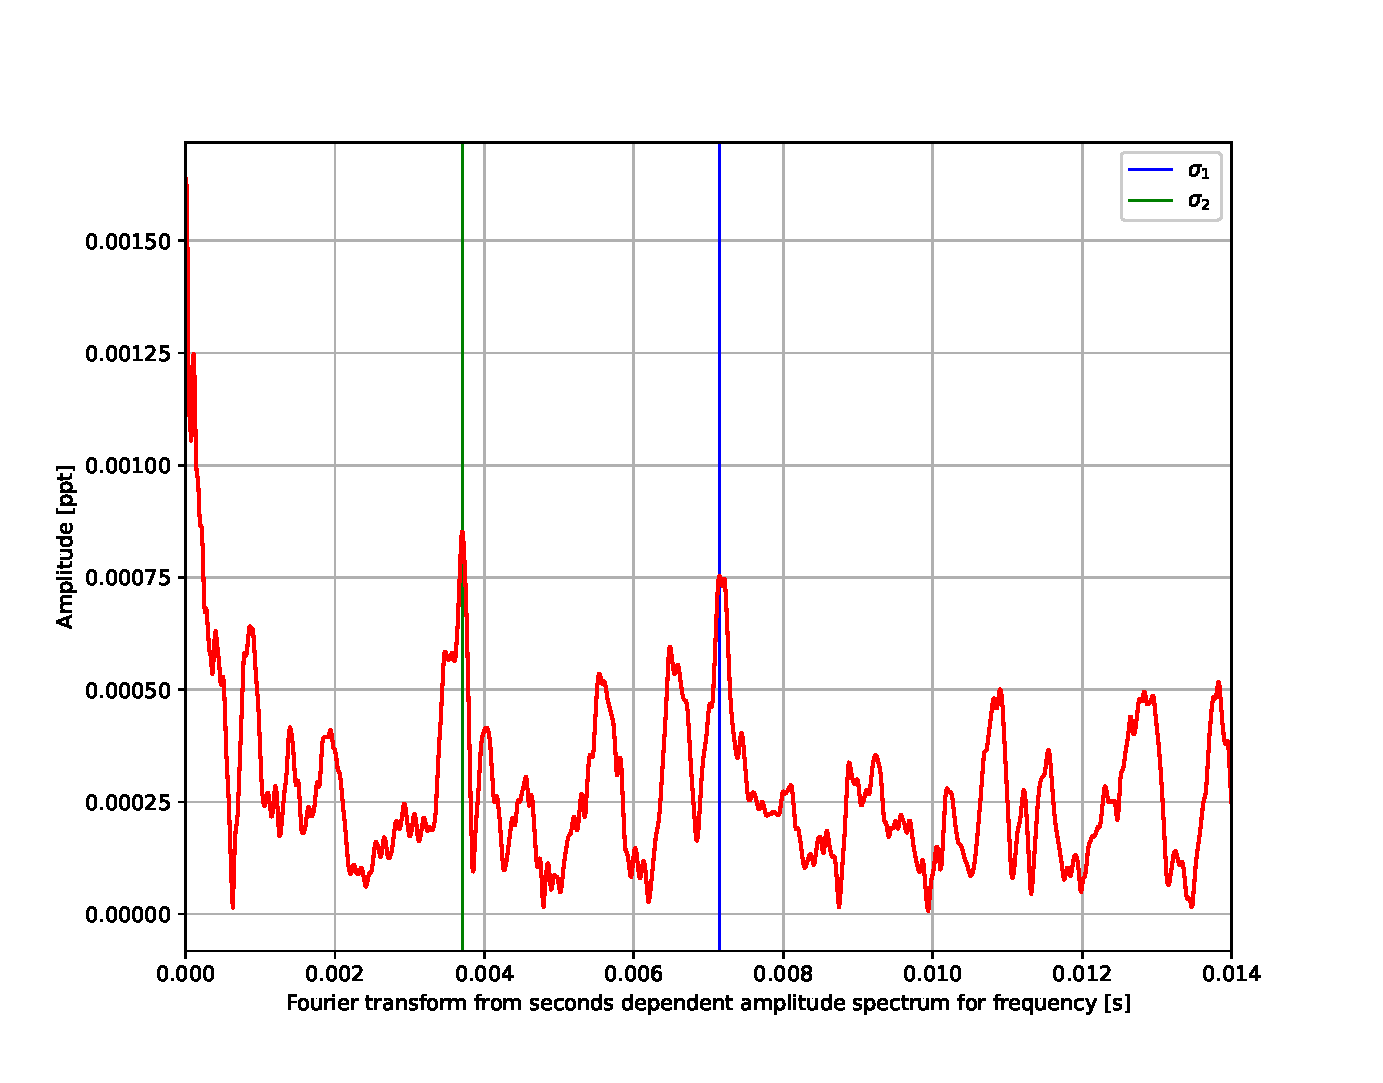
\includegraphics[scale=0.65]{images/2nd_ft.eps}
    \caption{Fourier transform confirming the determination of $ \Pi $ with marked maxima of $ \sigma_1 $, $ \sigma_2 $ histograms for each identified signal.}
    \label{fig:my_label_8}
\end{figure*}

\begin{table*}[b]
    \centering
    \begin{tabular}{c|c|c|c|c|c}
Index & Frequency [s] & Period [s] & Amplitude [ppt] & Numbers l and m & Number n \\ 
\hline 
0   &  11.687871 &  7392.278726 &  0.069794 &    2, -2  &   \\
1   &  11.691179 &  7390.186903 &  0.084929 &    2, -1  &   \\
2   &  11.692334 &  7389.456944 &  0.089297 &    2, 0  &  0 \\
3   &   11.69395 &   7388.43609 &  0.061972 &    2, +1  &   \\
4   &  11.696643 &  7386.734885 &  0.051378 &    2, +2  &      \\
5   &  11.697566 &  7386.151938 &  0.042368 &    2  &     1 \\
6   &  11.703568 &  7382.363789 &  0.045161 &    2  &         \\
7   &  12.139242 &  7117.412997 &  0.041216 &    2  &     3 \\
8  &  12.141089 &  7116.330081 &  0.185183 &    2  &      4 \\
9  &  12.143244 &  7115.067563 &  0.052738 &    2  &      5 \\
10  &  12.145706 &  7113.625072 &  0.072152 &    2  &     6 \\
11  &  12.616083 &  6848.401281 &  0.062762 &    2  &     7 \\
12  &  12.620316 &  6846.104573 &  0.045573 &    2  &     8 \\
13  &  12.621316 &  6845.561927 &  0.050248 &    2  &     9 \\
14  &  12.623162 &   6844.56067 &  0.089982 &    2  &     10  \\
15  &  12.624085 &  6844.060148 &  0.062989 &    2  &     11 \\
16  &   12.62524 &  6843.434085 &  0.046195 &    2  &     12 \\
17  &  12.626086 &  6842.975595 &  0.044561 &    2  &     13 \\
18  &  13.134321 &  6578.185398 &  0.064605 &    2  &     14 \\
19  &  13.136322 &  6577.183466 &  0.074395 &    2  &     15 \\
20  &  13.138092 &   6576.29736 &  0.104344 &    2  &     16 \\
21  &  13.141478 &  6574.603158 &  0.046138 &    2  &     17 \\
22  &  13.655638 &  6327.057121 &  0.043131 &    3  &         \\
23  &  13.656946 &   6326.45094 &   0.07842 &    3  &         \\
24  &  13.658408 &  6325.773764 &  0.174031 &    3  &         \\
25  &  14.255286 &  6060.909523 &  0.052377 &    2  &     18 \\
26  &  14.287989 &  6047.037274 &  0.091084 &    2  &         \\
27  &  14.290066 &  6046.158317 &  0.103591 &    2, -2  &      \\
28  &  14.921724 &  5790.215537 &  0.123525 &    2, -1  &      \\
29  &  14.923109 &  5789.678257 &  0.344852 &    2, 0  &    20     \\
30  &  14.924495 &  5789.140705 &  0.100397 &    2, +1  &         \\
31  &  16.334549 &  5289.402252 &  0.076301 &    2, +2  &      \\
32  &  16.339859 &  5287.683324 &  0.056953 &    2  &     21 \\
33  &  16.341013 &  5287.309928 &  0.051016 &    2  &     22 \\
34  &  16.342012 &  5286.986562 &  0.042326 &    2  &     23 \\
35  &  16.344091 &  5286.314043 &  0.041033 &    2  &         \\
36  &  17.187584 &  5026.884547 &  0.055428 &   2  &         \\
37  &  17.195433 &  5024.590059 &  0.065719 &   2  &         \\
38  &  17.196972 &  5024.140328 &  0.048017 &    2  &         \\
39  &   17.19828 &  5023.758093 &  0.038583 &    2  &         \\
40  &  17.199356 &  5023.443878 &  0.074763 &    2  &         \\
41  &  17.200357 &  5023.151426 &  0.116555 &    2, -2  &         \\
42  &  17.201973 &  5022.679678 &  0.244131 &    2, -1  &         \\
43  &  17.203358 &   5022.27539 &  0.660921 &    2, 0  &     30 \\
44  &  17.204742 &   5021.87117 &  0.100748 &    2, +1  &      \\
45  &  17.205744 &  5021.578901 &  0.083403 &    2, +2  &      \\
46  &  17.206591 &  5021.331753 &  0.112716 &    2  &     31 \\
47  &  17.208975 &  5020.636081 &  0.045892 &    2  &     32 \\
48  &  17.209591 &  5020.456352 &  0.053044 &    2  &     33 \\
49  &  17.211206 &  5019.985107 &  0.058084 &    2  &     34 \\
50  &  17.212208 &  5019.693061 &  0.037217 &    2  &     35 \\
51  &  17.218132 &  5017.965938 &  0.039706 &    2  &     36 \\
52  &  17.685892 &  4885.249749 &  0.039499 &    1  &     0 \\
53  &  17.691587 &  4883.677072 &   0.04821 &    1  &         \\
54  &  17.693665 &  4883.103766 &  0.044769 &    1  &         \\
55  &   17.69582 &  4882.509018 &   0.05444 &    1  &         \\
56  &  17.697973 &  4881.914939 &  0.076211 &    1  &         \\
57  &  17.699358 &  4881.532994 &  0.053501 &    1  &         \\
58  &  17.701668 &  4880.896028 &  0.065924 &    1  &         \\
59  &  17.703821 &  4880.302344 &  0.046614 &    1  &         \\
60  &  18.183971 &  4751.437299 &  0.047834 &    2  &     37 \\
    \end{tabular}
\end{table*}

\begin{table*}[]
    \centering
    \begin{tabular}{c|c|c|c|c|c}
Index & Frequency [s] & Period [s] & Amplitude [ppt] & Numbers l and m & Number n \\  
\hline 


61  &  18.185587 &  4751.015204 &  0.040378 &    2  &     38 \\
62  &  18.187281 &  4750.572758 &  0.065038 &    2, -2  &      \\
63  &  18.195129 &  4748.523528 &  0.069324 &    2, -1  &      \\
64  &  18.203054 &  4746.456169 &  0.672171 &    2 0 &     39   \\
65  &  18.210979 &  4744.390613 &  0.067572 &    2, +1  &         \\
66  &  18.217905 &  4742.587021 &  0.052674 &    2, +2  &         \\
67  &  18.218828 &  4742.346711 &  0.043955 &    2  &         \\
68 &  18.246452 &  4735.167058 &   0.04267 &    1  &     8 \\
69 &  20.232609 &  4270.334135 &  0.074524 &    1  &         \\
70 &  21.007235 &  4112.868817 &  0.040064 &    1  &         \\
71 &  21.008467 &  4112.627597 &  0.044996 &    1  &         \\
72 &  21.841496 &  3955.773082 &  0.117993 &    1  &     12 \\
73 &  22.045019 &  3919.252663 &  0.043751 &    2  &     41 \\
74 &  22.046482 &  3918.992592 &  0.201251 &    2  &     42 \\
75 &  22.705687 &  3805.214158 &  0.048795 &    1  &     13 \\
76 &  22.712612 &  3804.053864 &  0.040971 &    1  &     14 \\
77 &  22.713535 &  3803.899253 &  0.048534 &    1  &     15 \\
78 &  22.717461 &  3803.241982 &  0.039939 &    1  &     16 \\
79 &  22.718384 &  3803.087438 &  0.087243 &    1, -1  &      \\
80 &  22.721462 &  3802.572169 &  0.509853 &    1, 0  &      17   \\
81 &  22.724077 &  3802.134589 &  0.116377 &    1, +1  &         \\
82 &  23.616278 &  3658.493567 &  0.071092 &    1  &         \\
83 &  23.647057 &   3653.73169 &  0.046596 &    1  &     19 \\
84 &  23.670372 &  3650.132747 &  0.043553 &   2  &     43 \\
85 &  23.671988 &  3649.883639 &  0.045096 &   2  &     44 \\
86 &  23.678913 &  3648.816124 &  0.046307 &  1   &  20 \\
87 &  23.682299 &  3648.294502 &  0.052955 &  1   &  21 \\
88 &  23.683069 &  3648.175799 &  0.048491 &  1   &  22 \\
89 &  23.683992 &  3648.033599 &  0.061885 &  1   &  23 \\
90 &  23.684839 &  3647.903162 &  0.061257 &  1   &    24 \\
91 &  23.687763 &  3647.452874 &  0.042415 &  1  &     25 \\
92 &  23.688686 &  3647.310731 &  0.040786 &  1  &     26 \\
93 &  23.689301 &  3647.216171 &  0.062787 &  1   &     27 \\
94 &  23.690918 &  3646.967167 &  0.064309 &  1   &     28 \\
95 &  23.691763 &  3646.837101 &  0.087831 &  1, -1   &      \\
96 &   23.69969 &  3645.617326 &  0.996922 &  1, 0   &     29 \\
97 &  23.707615 &  3644.398661 &   0.08374 &  1, +1   &      \\
98 &  23.708538 &  3644.256756 &   0.05529 &  1   &     30 \\
99 &  23.709307 &  3644.138609 &   0.04838 &  1   &     31 \\
100 &  23.710077 &  3644.020175 &   0.06274 &  1   &     32 \\
101 &     23.711 &  3643.878301 &  0.047859 &  1   &     33 \\
102 &  23.712231 &  3643.689249 &  0.049148 &  1   &     34 \\
103 &  23.713078 &  3643.559121 &  0.043619 &  1   &     35 \\
104 &   23.71454 &  3643.334353 &  0.061614 &  1   &         \\
105 &  23.715464 &  3643.192531 &  0.087175 &  1   &         \\
106 &  23.724773 &  3641.762916 &  0.044907 &  1   &         \\
107 &  23.729082 &  3641.101649 &  0.050071 &  1   &         \\
108 &  23.877359 &  3618.490579 &  0.048206 &    1  &      \\
109 &  24.706541 &  3497.049619 &   0.05248 &    1, -1  &      \\
110 &  24.710619 &  3496.472513 &  0.152824 &    1, 0  &     41 \\
111 &  24.714005 &  3495.993534 &  0.048611 &    1, +1  &      \\
112 &  25.793957 &  3349.621805 &  0.047351 &   2  &         \\
113 &  25.802498 &  3348.513019 &  0.038077 &   2  &     46 \\
114 &  25.804806 &  3348.213538 &  0.228419 &   2  &     47 \\
115 &   26.95878 &  3204.892769 &  0.047304 &    1  &         \\
116 &  26.966476 &  3203.978102 &   0.04159 &    1  &         \\
117 &  31.044746 &  2783.079587 &  0.044616 &    2, -2 &         \\
118 &  31.070061 &  2780.812073 &  0.054514 &    2, -1  &      \\
119 &  31.073139 &  2780.536574 &  0.089261 &    2, 0  &     48 \\
120 &  31.073986 &  2780.460796 &   0.06578 &    2, +1  &      \\
    \end{tabular}
\end{table*}

\begin{table*}[]
    \centering
    \begin{tabular}{c|c|c|c|c|c}
Index & Frequency [s] & Period [s] & Amplitude [ppt] & Numbers l and m & Number n \\ 
\hline 

121 &  31.075064 &  2780.364372 &  0.073978 &    2, +2  &      \\
122 &  31.076372 &  2780.247308 &  0.493493 &    2  &         \\
123 &  31.077757 &  2780.123428 &  0.103449 &    2  &         \\
124 &  31.078833 &  2780.027198 &  0.057261 &    2  &         \\
125 &  31.079603 &  2779.958272 &  0.059969 &    2  &         \\
126 &   31.08045 &  2779.882525 &  0.069354 &    2  &         \\
127 &  31.081911 &  2779.751855 &  0.041901 &    2  &         \\
128 &  31.084297 &  2779.538476 &  0.060012 &    2  &         \\
129 &  31.092222 &  2778.830005 &  0.047492 &    2  &         \\
130 &  34.404331 &  2511.311715 &  0.038026 &    2  &     57 \\
    \end{tabular}
    \label{tab:my_label}
\end{table*}

\end{document}